\chapter{Memory architecture and data locality}
\begin{center}
      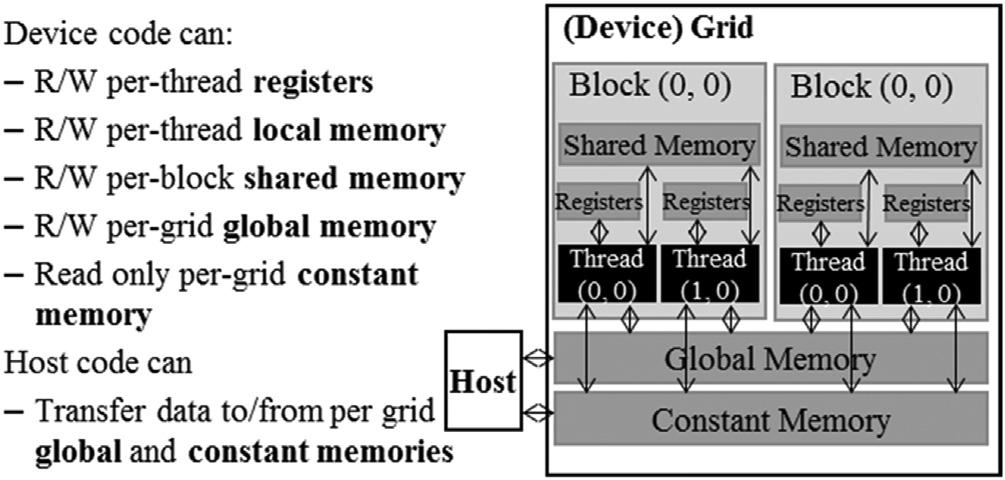
\includegraphics[width=0.8\linewidth]{Images/Memories/memory_types.png}
\end{center}
\begin{itemize}
      \item \textbf{Global memory}:
            \begin{itemize}
                  \item Can be both read and written by \textsl{Device}.
                  \item Can be both read and written by \textsl{Host}.
            \end{itemize}
      \item \textbf{Constant memory}:
            \begin{itemize}
                  \item Offers short-latency high-bandwidth \textbf{\textsl{read-only access}} to \textsl{Device}.
                  \item Can be both read and written by \textsl{Host}.
            \end{itemize}
      \item \textbf{Local memory}:
            \begin{itemize}
                  \item Resides in the global memory, but is not shared across threads. Each thread has its own private local memory, where places the data that is private to the thread but cannot be allocated in the registers. This data includes statically allocated arrays, spilled registers, and other elements of the thread's call stack.
            \end{itemize}
      \item  \textbf{Registers and Shared memory}:
            \begin{itemize}
                  \item Are on-chip memories. Variables that reside in registers/shared memory can be accessed at very high speed in highly parallel manner.
                  \item Registers are allocated to individual threads; each thread can access its own set of registers.
                  \item \textsl{Kernel function typically uses registers} to store frequently accessed variables that are private to each thread.
                  \item \textsl{Shared memory is allocated to thread blocks}; all threads in a block can access shared memory variables declared for the block.
                        \begin{itemize}
                              \item Shared memory is an efficient means by which threads can cooperate by sharing their input data and intermediate results.
                              \item By declaring a CUDA variable in one of the CUDA memory types, a CUDA programmer dictates the visibility
                                    and access speed of the variable.
                        \end{itemize}
            \end{itemize}
\end{itemize}

\begin{tcolorbox}
      \subsubsection{CPU vs GPU Register architecture}
      \begin{itemize}
            \item When CPUs context switch between different threads, they save the registers of the outgoing thread to memory and restore the registers of the incoming thread from memory.
            \item In contrast, GPUs achieve zero-overhead scheduling by keeping the registers of all the threads that are scheduled on the processing block in the processing block's register file.
            \item This way, switching between warps of threads is instantaneous because the registers of the incoming threads are already in the register file. Consequently, GPU register files need to be substantially larger than CPU register files
      \end{itemize}
\end{tcolorbox}
\section{- Advantages of Registers over Global Memory}
\begin{itemize}
      \item Global memory is implemented with DRAM technology, implying long access latencies and relatively low access bandwidths.
      \item The registers on the other hand, are on the processor chip, which implies very short access latency and very large access bandwidth, compared to the global memory.
            \begin{itemize}
                  \item Floating-point addition with operands on global memory:
                        \begin{center}
                              \texttt{load r2, r4, offset}\\
                              \texttt{fadd r1, r2, r3}
                        \end{center}
                        \texttt{load} instruction adds an offset value to the contents of \texttt{r4} to form an address for the operand value. It then accesses the global memory and places the value into register \texttt{r2}. Once the operand value is in \texttt{r2}, the \texttt{fadd} instruction performs the floating-point addition using the values in \texttt{r2} and \texttt{r3} and places the result into \texttt{r1}.\\
                        Since the processor can fetch and execute only a limited number of instructions per clock cycle, the version with an additional load will likely take more time to process than the one without.
            \end{itemize}
      \item Whenever a variable is stored in a register, its accesses no longer consume off-chip global memory bandwidth. \textsl{A subtler point is that each access to registers involves fewer instructions than access to the global memory.}
            \begin{itemize}
                  \item Floating-point addition with operands on built-in registers:
                        \begin{center}
                              \texttt{fadd r1, r2, r3}
                        \end{center}
                        The register files \texttt{r2} and \texttt{r3} are the files where input values can be found. The addition of \texttt{r2} and \texttt{r3} are stored in \texttt{r1}.
            \end{itemize}
      \item In modern computers the energy that is consumed for accessing a value from the register file is at least an order of magnitude lower than for accessing a valuefrom the global memory. Accessing a value from registers has a tremendous advantage
            in energy efficiency over accessing the value from the global memory.
\end{itemize}

\section{Shared memory vs Registers}
\begin{center}
      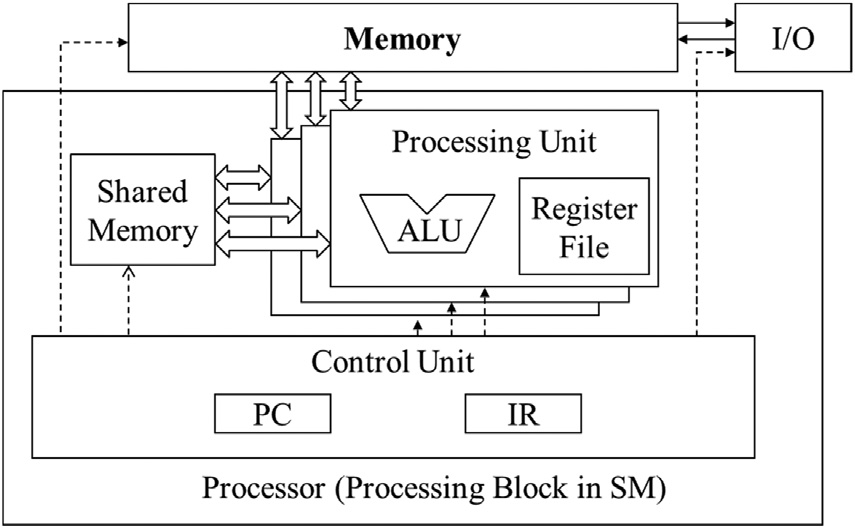
\includegraphics[width=0.5\linewidth]{Images/Memories/CUDA_device_SM.png}
\end{center}
\begin{itemize}
      \item Shared memory
            \begin{itemize}
                  \item Is designed as part of the memory space that resides on the processor chip.
                  \item When the processor needs to access the data, it still has to perform the \texttt{load} operation same as when accessing the data from the global memory.
                  \item However, as the shared memory resides on-chip, it can be accessed with much lower latency and much higher throughput than in global memory access.
                  \item Because of the need to perform a load operation, shared memory has longer latency and lower bandwidth than registers.
                  \item In computer architecture terminology the shared memory is a form of \textsl{scratchpad memory}.
            \end{itemize}
      \item One important difference between \textsl{Shared Memory} and the \textsl{Registers} is that, \textsl{Shared Memory is accessible by all the threads in a block}. This is contrary to the \textsl{register data, which is private to a thread}.
      \item CUDA device SM typically employs multiple processing units to allow multiple threads to make simultaneous progress.
      \item Threads in a block can be spread across these processing units.
      \item Therefore, the hardware implementations of the shared memory in these CUDA devices are typically designed to allow multiple processing units to simultaneously access its contents to support efficient data sharing among threads in a block.
\end{itemize}

\section{- Declaring program variables into the various memory types}
\begin{center}
      \begin{tabular}{c|c|c|c}
            Variable declaration                          & Memory   & Scope  & Lifetime    \\
            \hline
            Automatic variables other than arrays         & Register & Thread & Grid        \\
            Automatic array variables                     & Local    & Thread & Grid        \\
            \_\_device\_\_ \_\_shared\_\_ int SharedVar;  & Shared   & Block  & Grid        \\
            \_\_device\_\_ int GlobalVar;                 & Global   & Grid   & Application \\
            \_\_device\_\_ \_\_constant\_\_ int ConstVar; & Constant & Grid   & Application \\
      \end{tabular}
\end{center}
\begin{enumerate}
      \item If a variable's scope is a single thread, a private version of the variable will be created for every thread; each thread can access only its private version of the variable.
      \item Lifetime tells the portion of the program's execution duration when the variable is available for use: either within a grid's execution or throughout the entire application.
      \item If a \textbf{variable's lifetime is within a grid's execution, it must be declared within the kernel function body and will be available for use only by the kernel's code}. If the kernel is invoked several times, the value of the variable is not maintained across these invocations. Each invocation must initialize the variable in order to use it.
      \item If a variable's lifetime is throughout the entire application, it must be declared outside of any function body. The contents of these variables are maintained throughout the execution of the application and available to all kernels.
      \item Variables that are not arrays are \textsl{scalar} variables. \textbf{All automatic scalar variables that are declared in kernel and device functions are placed into registers.} The scopes of these automatic variables are within individual threads. When a \textbf{kernel function declares an automatic variable, a private copy of that variable is generated for every thread that executes the kernel function. When a thread terminates, all its automatic variables cease to exist.}
      \item Automatic array variables are not stored in registers. They are stored in thread's local memory and may incur access delays. A private version of each automatic array is created for and used for every thread. Once a thread terminates its execution, the contents of its automatic array variables cease to exist.
      \item If a variable declaration is preceded by \texttt{\_\_shared\_\_} keyword, it is declared as a shared variable in CUDA. Such a declaration is typically made within a kernel function or a device function.
            \begin{itemize}
                  \item \textbf{Shared variables reside in the shared memory. The scope of a shared variable is within a thread block}; that is, all threads in a block see the same version of a shared variable.
                  \item \textbf{A private version of the shared variable is created for and used by each block during kernel execution. The lifetime of a shared variable is within the duration of the kernel execution.} When a kernel terminates its grid's execution, the contents of its shared variables cease to exist.
                  \item Accessing shared variables from the shared memory is extremely fast and highly parallel. CUDA programmers often use shared variables to hold the portion of global memory data that is frequently used and reused in an execution phase of the kernel.
            \end{itemize}
      \item If a variable declaration is preceded by the \texttt{\_\_constant\_\_} keyword, then the variable is declared as a constant in CUDA.\textbf{ Declaration of constant variables must be outside any function body}.
            \begin{itemize}
                  \item The scope of a constant variable is all grids, meaning that all threads in all grids see the same version of a constant variable. The lifetime of a constant variable is the entire application execution.
                  \item Constant variables are \textbf{stored in the global memory but are cached for efficient access}. Currently, the total size of constant variables in an application is limited to 65,536 bytes.
            \end{itemize}
      \item If a variable declaration is preceded by the \texttt{\_\_device\_\_} keyword, \textbf{the global variable is placed in the global memory.}
            \begin{itemize}
                  \item Accesses to the global variable are slow.
                  \item One important advantage of global variables is that they are visible to all threads of all kernels. Their contents also persist through the entire execution.
                  \item Thus, global variables can be used as a means for threads to collaborate across blocks.
                  \item \textsl{There is currently no easy way to synchronize between threads from different thread blocks or to ensure data consistency across threads in accessing global memory other than using atomic operations or terminating the current kernel execution.}
                  \item \textbf{Therefore, global variables are often used to pass information from one kernel invocation to another kernel invocation.}
            \end{itemize}
      \item In CUDA, pointers can be used to point to data objects in the global memory.
            \begin{itemize}
                  \item If an object is allocated by a host function, the pointer to the object is initialized by memory allocation API functions such as \texttt{cudaMalloc} and \texttt{cudaMemCpy} functions and can be passed to the kernel function as a parameter.
                  \item Assign the address of a  variable is declared in the global memory to a pointer variable in a kernel function.\\
                        \texttt{float* ptr = \&GlobalVar;}, where \texttt{float *ptr} is an automatic pointer variable which points to the global variable.
            \end{itemize}
\end{enumerate}

\pagebreak
\section{Q \& A}
\begin{enumerate}
      \item Consider matrix addition. Can one use shared memory to reduce the global memory bandwidth consumption? Hint: Analyze the elements that are accessed by each thread and see whether there is any commonality between threads.
            \\ \textsl{A:} No, the use of shared memory has no effect here. There is no commonality between the elements accessed by any two or more given threads.
      \item What type of incorrect execution behavior can happen if one forgot to use one or both \texttt{\_\_syncthreads()} in the kernel?
            \begin{center}
                  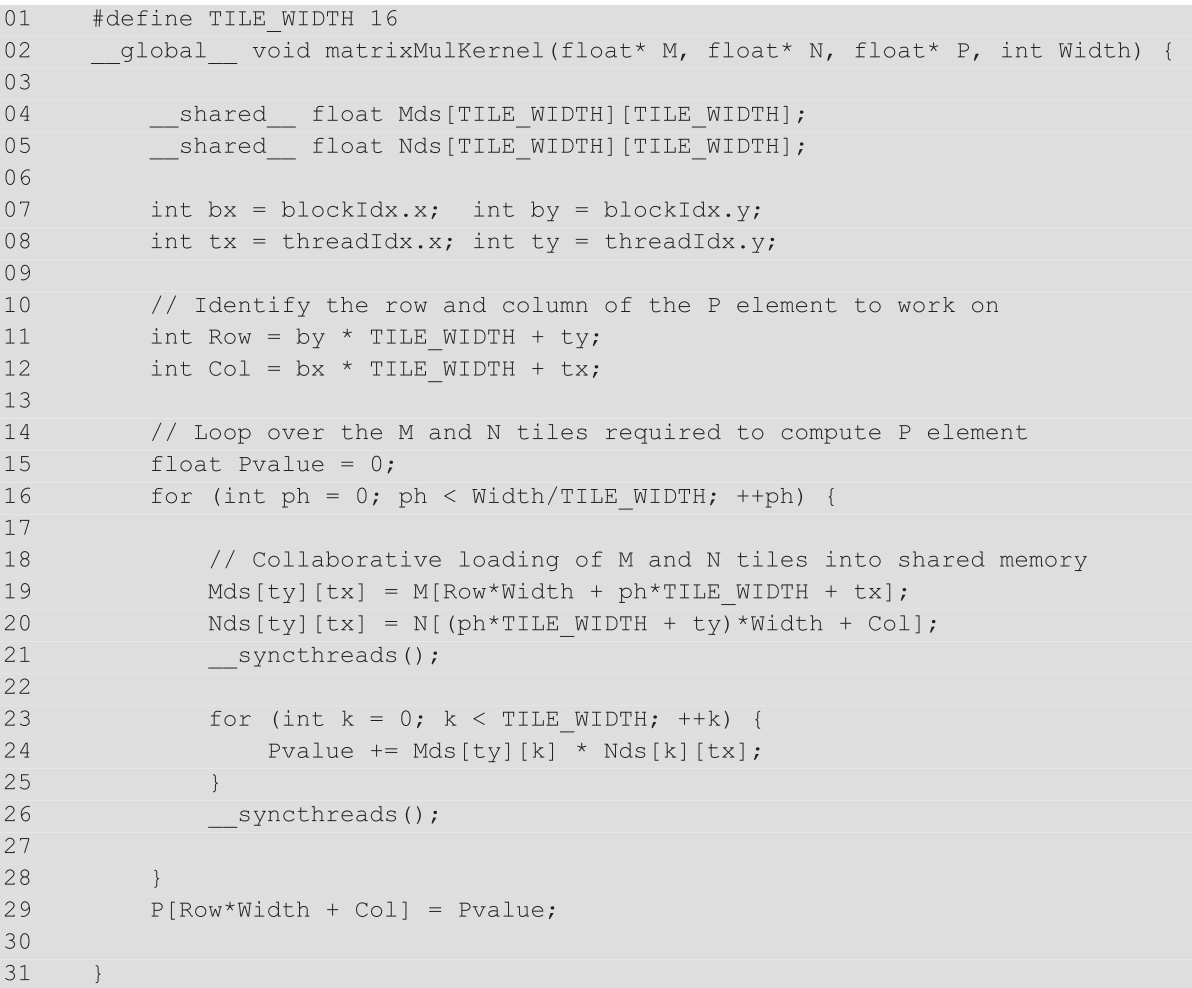
\includegraphics[width=0.9\linewidth]{Images/Memories/tiled_kernel.png}
            \end{center}
            \textsl{A:} If the \texttt{\_\_syncthreads()} in \texttt{line 21} is not used, the loading of elements from global memory into the shared memory \texttt{Mds} and \texttt{Nds} is not synchronized/ensured for the entire block. This would in turn pass wrong and incomplete values of \texttt{Mds} and \texttt{Nds} during the calculation of \texttt{Pvalue} in \texttt{line 24}.\\
            If the \texttt{\_\_syncthreads()} in \texttt{line 26} is not used, the threads that write might get ahead of the other thread and write false values into the output matrix \texttt{P}.
      \item Assuming that capacity is not an issue for registers or shared memory, give one important reason why it would be valuable to use shared memory instead of registers to hold values fetched from global memory? Explain your answer.
            \\\textsl{A:} The values stored in the shared memories can be accessed by all the threads in the block. By loading the values from the global memory into shared memory, the loaded data can be reused by multiple threads with single variable/memory fetch.\\ If the data is directly loaded into registers directly, the data is restricted to a thread. If the same values are required by multiple threads, then they need to be loaded so many times, once per each thread.

      \item For our tiled matrix-matrix multiplication kernel, if we use a 32 3 32 tile, what is the reduction of memory bandwidth usage for input matrices M and N?
            \\\textsl{A:} 32$\times$ reduction.
      \item Assume that a CUDA kernel is launched with 1000 thread blocks, each of which has 512 threads. If a variable is declared as a local variable in the kernel, how many versions of the variable will be created through the lifetime of the execution of the kernel?
            \\\textsl{A:} 512,000 instances. 1 instance of the variable per thread.
      \item In the previous question, if a variable is declared as a shared memory variable, how many versions of the variable will be created through the lifetime of the execution of the kernel?
            \\\textsl{A:} 1,000 instances. 1 per thread block.
      \item Consider performing a matrix multiplication of two input matrices with dimensions N$\times$N. How many times is each element in the input matrices requested from global memory when:
            \begin{itemize}
                  \item a. There is no tiling?
                        \\ \textsl{A:} N times.
                  \item b. Tiles of size T$\times$T are used?
                        \\ \textsl{A: } N / T times.
            \end{itemize}

      \item A kernel performs 36 floating-point operations and seven 32-bit global memory accesses per thread. For each of the following device properties, indicate whether this kernel is compute-bound or memory-bound.
            \begin{itemize}
                  \item[ a.] Peak FLOPS=200 GFLOPS, peak memory bandwidth=100 GB/second
                        \\ \textsl{A:}
                        \begin{equation*}
                              \begin{aligned}
                                    \text{computational intensity}         & = \frac{\text{Floating point operations} }{\text{Num. Memory accesses} \times  \text{\text{size of access(bytes)}}} \\
                                                                           & = \frac{36}{7\times4}                                                                                               \\
                                                                           & = 1.286 \text{ FLOP/Byte}                                                                                           \\\\
                                    \text{memory bandwidth limit}          & = \text{peak memory bandwidth}                 \times \text{computational intensity}                                \\
                                                                           & = 100 \times 1.286 = \textbf{128.6 GFLOPS.}                                                                         \\\\
                                    \text{ 128.6 (memory bandwidth limit)} & > \text{100 (peak memory bandwidth)}                                                                                \\
                                    \implies                               & \textbf{The kernel is memory bound.}                                                                                \\
                              \end{aligned}
                        \end{equation*}
                  \item[ b.] Peak FLOPS=300 GFLOPS, peak memory bandwidth=250 GB/second
                        \\ \textsl{A: }
                        \begin{equation*}
                              \begin{aligned}
                                    \text{computational intensity}        & = 1.286 \text{ FLOP/Byte}                          \\
                                    \text{memory bandwidth limit}         & = 250 \times 1.286 = \textbf{321.5 \text{ GFLOPS}} \\\\
                                    321.5 (\text{memory bandwidth limit}) & > 300 (\text{Peak FLOPS})                          \\
                                    \implies                              & \textbf{The kernel is compute bound.}              \\
                              \end{aligned}
                        \end{equation*}
            \end{itemize}
            \pagebreak
      \item To manipulate tiles, a new CUDA programmer has written a device kernel that will transpose each tile in a matrix. The tiles are of size BLOCK\_WIDTH by BLOCK\_WIDTH, and each of the dimensions of matrix A is known to be a multiple of BLOCK\_WIDTH. The kernel invocation and code are shown below. BLOCK\_WIDTH is known at compile time and could be set anywhere from 1 to 20.
            \begin{center}
                  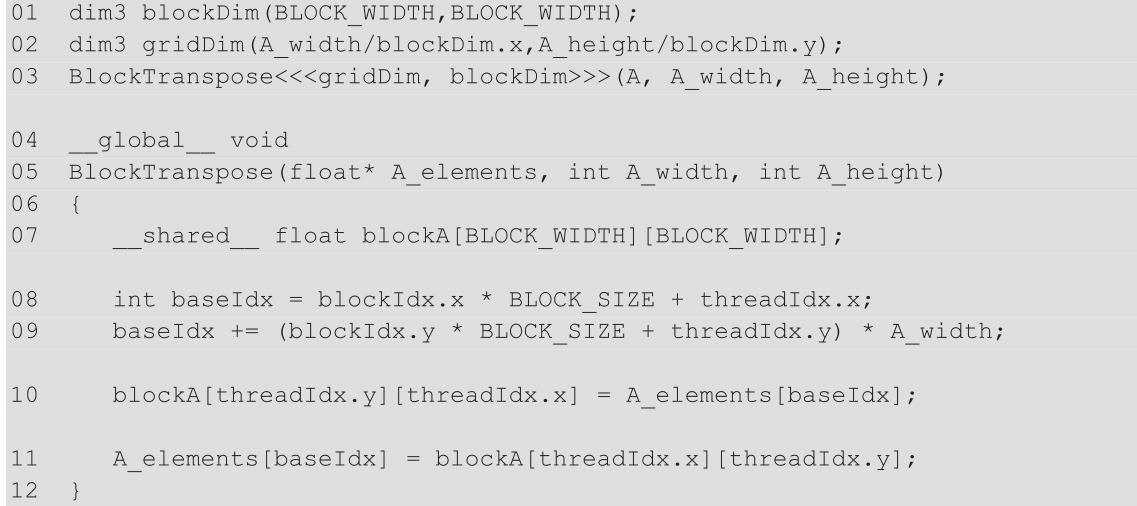
\includegraphics[width=0.9\linewidth]{Images/Memories/blocktranspose.png}
            \end{center}
            \begin{itemize}
                  \item[a.] Out of the possible range of values for BLOCK\_SIZE, for what values of BLOCK\_SIZE will this kernel function execute correctly on the device?
                        \\ \textsl{A: }
                        \\\textbf{ After loading the elements of \texttt{A\_elements} into the shared memory \texttt{blockA}, there is no barrier function such as \texttt{\_\_syncthreads()} to ensure the completion of write operations of all the threads into the shared memory.}
                  \item[b.] If the code does not execute correctly for all BLOCK\_SIZE values, what is the root cause of this incorrect execution behavior? Suggest a fix to the code to make it work for all BLOCK\_SIZE values.
                        \\\textsl{A:} Placement of \texttt{\_\_syncthreads()} directly after line 10.
            \end{itemize}
      \item Consider the following CUDA kernel and the corresponding host function that calls it:
            \begin{center}
                  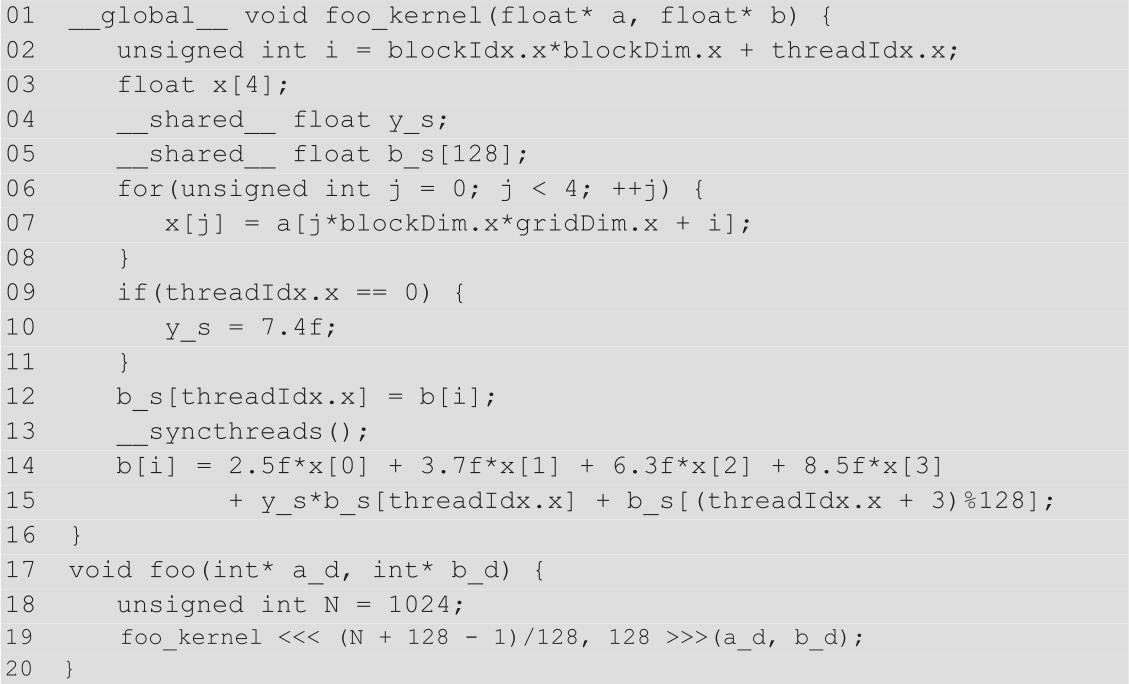
\includegraphics[width=0.8\linewidth]{Images/Memories/foo_kernel.png}
            \end{center}
            \begin{itemize}
                  \item[a.] How many versions of the variable \texttt{i} are there?
                        \\\textsl{A:} \textbf{Automatic variable.} Each thread has a unique \texttt{i} \(\implies\) \textbf{1024 versions.}
                  \item[b.] How many versions of the array \texttt{x[]} are there?
                        \\\textsl{A:} \textbf{Automatic variable.} Each thread has a unique \texttt{x[]} \(\implies\) \textbf{1024 versions.}
                  \item[c.] How many versions of the variable \texttt{y\_s} are there?
                        \\\textsl{A:} \textbf{Shared variable}. Each block has a unique \texttt{y\_s} \(\implies\) (1024 + 128 - 1) / 128 = \textbf{8 versions}
                  \item[d.] How many versions of the array \texttt{b\_s[]} are there?
                        \\\textsl{A:} \textbf{Shared variable}. Each block has a unique \texttt{y\_s} \(\implies\) (1024 + 128 - 1) / 128 = \textbf{8 versions}
                  \item [e.] What is the amount of shared memory used per block (in bytes)?
                        \\\textsl{A:} \texttt{\_\_shared\_\_ float y\_s} uses 4 bytes + \texttt{\_\_shared\_\_ float b\_s[128]} uses 4 \(times\) 128 bytes of shared memory. (4: \texttt{sizeof(float)}) $\implies$ 516 bytes.
                  \item [f.] What is the floating-point to global memory access ratio of the kernel (in OP/B)?
                        \\\textsl{A:}
                        \begin{equation*}
                              \begin{aligned}
                                    \text{In line 14,}                &                                                               \\
                                    \text{FLOPs per thread}           & = \text{5 Multiplications + 1 Modulo operation + 5 Additions} \\
                                    \text{Global Memory access count} & = \text{4 (line 06) + 1 (line 12) + 1 (line 14)}              \\
                                    \text{FLOP to GMEM ratio}         & = 11 / 6 = \textbf{1.83}
                              \end{aligned}
                        \end{equation*}
            \end{itemize}

            % \item Consider a GPU with the following hardware limits: 2048 threads/SM, 32 blocks/SM, 64K (65,536) registers/SM, and 96 KB of shared memory/SM. For each of the following kernel characteristics, specify whether the kernel can achieve full occupancy. If not, specify the limiting factor.
            %       \begin{itemize}
            %             \item [a.] The kernel uses 64 threads/block, 27 registers/thread, and 4 KB of shared memory/SM.
            %                   \\\textsl{A:}
            %                   \begin{equation*}
            %                         \begin{aligned}
            %                               \text{number of blocks}                & = 2048 / 64 = \text{32 blocks.} \textcolor{ForestGreen}{~<\text{ max blocks/SM}}   \\
            %                               \implies \text{Occupancy of blocks}    & = 32/ 32 = 100\%                                                                   \\
            %                               \text{registers occupied}              & = 27 \times 2048 = 55,296 reg. \textcolor{ForestGreen}{~< \text{max registers/SM}} \\
            %                               \implies \text{Occupancy of registers} & = 55,296/65,536 = 84.37\%                                                          \\
            %                               \text{SHMEM used}                      & = 4 \text{KB/SM} \textcolor{ForestGreen}{~<\text{ max SHMEM/SM}}                   \\
            %                               \implies \text{Occupancy of SHMEM}     & = 4/96 = 4.1\%
            %                         \end{aligned}
            %                   \end{equation*}
            %                   Full occupancy is not reached, is limited by shared memory.

            %             \item [b.] The kernel uses 256 threads/block, 31 registers/thread, and 8 KB of shared memory/SM.
            %       \end{itemize}
\end{enumerate}